% Metódy inžinierskej práce

\documentclass[10pt,twoside,english,a4paper]{article}

\usepackage[english]{babel}
\usepackage[T1]{fontenc}
\usepackage[IL2]{fontenc} % lepšia sadzba písmena Ľ než v T1
\usepackage[utf8]{inputenc}
\usepackage{graphicx}
\usepackage{url} % príkaz \url na formátovanie URL
\usepackage{hyperref} % odkazy v texte budú aktívne (pri niektorých triedach dokumentov spôsobuje posun textu)

\usepackage{cite}
\usepackage{times}
\usepackage{ragged2e}

\pagestyle{headings}

\title{Application of vector algebra and physics in 
designing steering behaviours of autonomous agents for 
realistic display in two dimensions\thanks{Semestrálny projekt v 
predmete Metódy inžinierskej práce, ak. rok 2022/23, 
vedenie: Mirwais Ahmadzai}} 

\author{Richard Čerňanský\\
		Dominik Zaťovič\\[2pt]
	{\small Slovenská technická univerzita v Bratislave}\\
	{\small Fakulta informatiky a informačných technológií}\\
	{\small \texttt{xcernansky@stuba.sk}}\\
	{\small \texttt{xzatovic@stuba.sk}}
	}

\date{\small November 3, 2022 } 

\begin{document}

\maketitle

\begin{abstract}

    In this article, we will focus on the problem of animating steering 
    behaviors of software-based autonomous agents in 
    games. As we want the player to have the best realistic experience 
    from the movement of the objects possible, we need to design 
    their behavior according to the physics that describes it. 
    The objective of this article is to explain my ideas on how to calculate 
    the steering force in the seek and arrive steering behavior and create 
    an algorithm that animates such motion. The algorithm will be written 
    in the p5.js library of JavaScript language. 

\end{abstract}

\section{Introduction}

\subsection{Motives and contents of the article} \label{motives}
Development in animation and games forces the creators to make 
the games more and more realistic. One of the most important 
aspects of the realistic perception of a game is the movement of 
objects and the animation itself. Jonathan Cooper in the chapter 
\textbf{The 12 principles of animation in video games}\cite{Cooper} 
of his book mentions 12 basic principles of a well-animated game. 
The sixth one named Slow In and Slow Out says:\emph{"Objects that burst into full 
speed immediately can look weightless and unrealistic, so it is here 
again that there is a conflict between the gameplay desire to give 
objects the ability to move immediately versus the artistic desire to give weight 
to a character."} That is why I came up with some ideas on how to 
design steering motion animations on the objects that look as realistic as possible.

In this article, we will call the objects autonomous agents. 
More about them will be explained in part \ref{definition of a.a.}. 
After understanding the concept of autonomous agents, we will state 
a problem in part \ref{problem to solve}. In part \ref{seek and 
arrive} we will have a closer look at the problem and derive some 
formulas necessary for the simulation. Finally, we will simulate 
the steering behavior, stated as a problem in p. \ref{problem to 
solve} by writing the code in p5.js (in p. \ref{class Vehicle}). 

\subsection{A brief history of steering animation in video games} \label{history}
Animation in games has a long history of depicting the steering movements of 
objects. The early days of gaming saw the introduction of simple animations, 
such as the moving dots in the game Pong, which were controlled by the player. 
As technology advanced, so did the ability to create more complex animations, 
including the steering movements of objects. 

One of the major developments in 
the history of animation in games was the introduction of 3D graphics in the 
1990s, which allowed for more realistic and dynamic depictions of steering 
movements. Today, animation in games plays a crucial role in creating a lifelike 
and immersive gaming experience, with many games featuring highly detailed 
animations of objects and characters moving and steering in a realistic manner.

\section{Autonomous agents} \label{autonomous agents} 

The term autonomous agent can be obscure so at first we need to 
understand it.

\subsection{Definition of autonomous agents} \label{definition of a.a.}

Autonomous agents generally refer to an entity that chooses 
how to act in its environment without any influence from a global 
plan or a leader. In games, these agents are not controlled by a 
player, but they are an important part of the game because their actions
can significantly influence the flow of the game. For example, 
a villain who runs away from the police decides on his own that he
wants to escape and starts an action. There are three key 
components of autonomous agents we want to keep in mind 
\cite{Verhagen}. 

\begin{enumerate}
    \item An autonomous agent has a limited ability to perceive its 
    environment. It makes sense that if an autonomous agent must decide 
    on its action, it should be somehow aware of the environment it 
    is located in. The question here is how limited the ability is. 
    If we wanted the object to be an all-knowing creature aware of 
    everything else around it, we need to give it access to 
    information about everything. On the other side if we wanted it 
    to have just a very narrow view of the environment, let’s say just 
    a few pixels around it.
    
    \item An autonomous agent processes the information from its 
    environment and calculates an action. The action is represented 
    as a force that influences the object. For example, a police 
    officer sees a thief and is attracted to him. The attraction is 
    represented by a force pointing toward his location. 
    
    \item An autonomous agent should have no leader. This is not 
    something that defines every autonomous agent. Sometimes you need 
    to state some global rules that it must follow, but mostly you want 
    the object to decide on its own\footnote{however, the designer can 
    include some specific attributes if needed}, calculate its own 
    actions.

\end{enumerate}

\subsection{Types of behaviors according to the number of objects 
involved} \label{types of behaviors}

Craig Raynolds in his paper from Game Developers Conference 
\textbf{Steering Behaviors For Autonomous Characters} \cite{Raynolds} 
introduces some types of behaviors that could appear talking about 
autonomous agents and how they behave. They divide into two main 
groups:

\begin{itemize}

\item Simple behavior for individuals and pairs\newline
Containing only one or two autonomous agents.

\item Combined behaviors and groups\newline
Containing more than two autonomous agents.

\end{itemize}

In this article, we will focus on the first mentioned because 
the combined behaviors are just more complicated kinds but 
the basic ideas are derived from the simple behaviors for 
individuals and groups. 

\section{Problem statement} \label{problem}

Now as we have explained what it takes for the object to behave like 
an autonomous agent we should understand more specific self-operating
concept of a vehicle to be able to grasp a problem we state later 
in this chapter.

\subsection{Braitenberg vehicle} \label{braitenberg}

Braitenberg vehicle is an entity that is a hypothetical self-operating
machine that can make decisions about how to behave in an environment
based on its sense perception. Valentino Braitenberg explains his 
concept in the book \textbf{Vehicles} \cite{Braitenberg}. Here is 
an example of that type of vehicle from the book:

\bigbreak

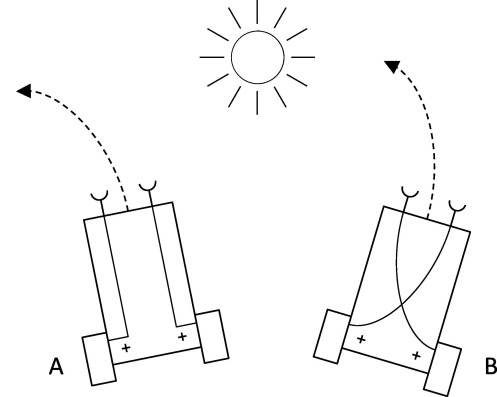
\includegraphics[scale=0.33]{braitenberg.jpg}
\quad Figure 1
\bigbreak

Vehicle A steers away from the light source and vehicle B steers 
toward the light source. It is not just about steering away or 
towards the sun. We could say that these vehicles feel emotion about 
the object. Vehicle A feels fear of the sun and vehicle B is 
attracted to it. We want the term vehicle to be clear because in 
the paper when we mention vehicle, we will be referring to the 
concept of the Braitenberg vehicle and its characteristics. 

\subsection{Problem to solve} \label{problem to solve}

Our goal is to animate a simple steering behavior. The best way to represent
it is by steering a car. It is also a frequently occurring situation 
in many games to steer a self-controlled car realistically.
Let’s simulate a simple behavior for a pair 
(p. \ref{types of behaviors}). The car that 
is expected to arrive at a specific position (f. e. a parking lot). 
We could say that in the car there is a driver or a device that decides on its own.
It perceives the environment with its "eyes" and sees the location of the parking 
lot. Processes its distance from the place and calculates and action \ref{definition of a.a.}. 
It starts \textbf{steering} towards the parking lot (attraction towards the 
parking lot is based on the same emotional principle as vehicle B in part \ref{braitenberg}). 
Notice the word steering here which is very important. We do not want 
to simulate an unrealistically moving car that is immediately able to 
turn around and head toward the target at a maximum speed. We want the 
animation to be smooth and realistically looking. What rules do we 
have to follow if we want to simulate a situation like this?

\section{Seek and arrive – a pursuit of a static target} \label{seek and arrive}

In the language of steering behaviors, the problem can be translated as 
a designing a seek and arrival behavior on one object and a target. 
If we want to write an algorithm we need to come up with some 
formulas to calculate the motion.

\subsection{Simple vehicle model} \label{model}
To describe an agent using physics, it is important to have some
mathematical variables that describe it. Craig Raynolds in his 
paper \cite{Raynolds} presents a simple 
vehicle model which needs to be introduced. There are six 
attributes that our vehicle will possess:
\newline 
\newline
\textbf{Simple Vehicle Model:} \\
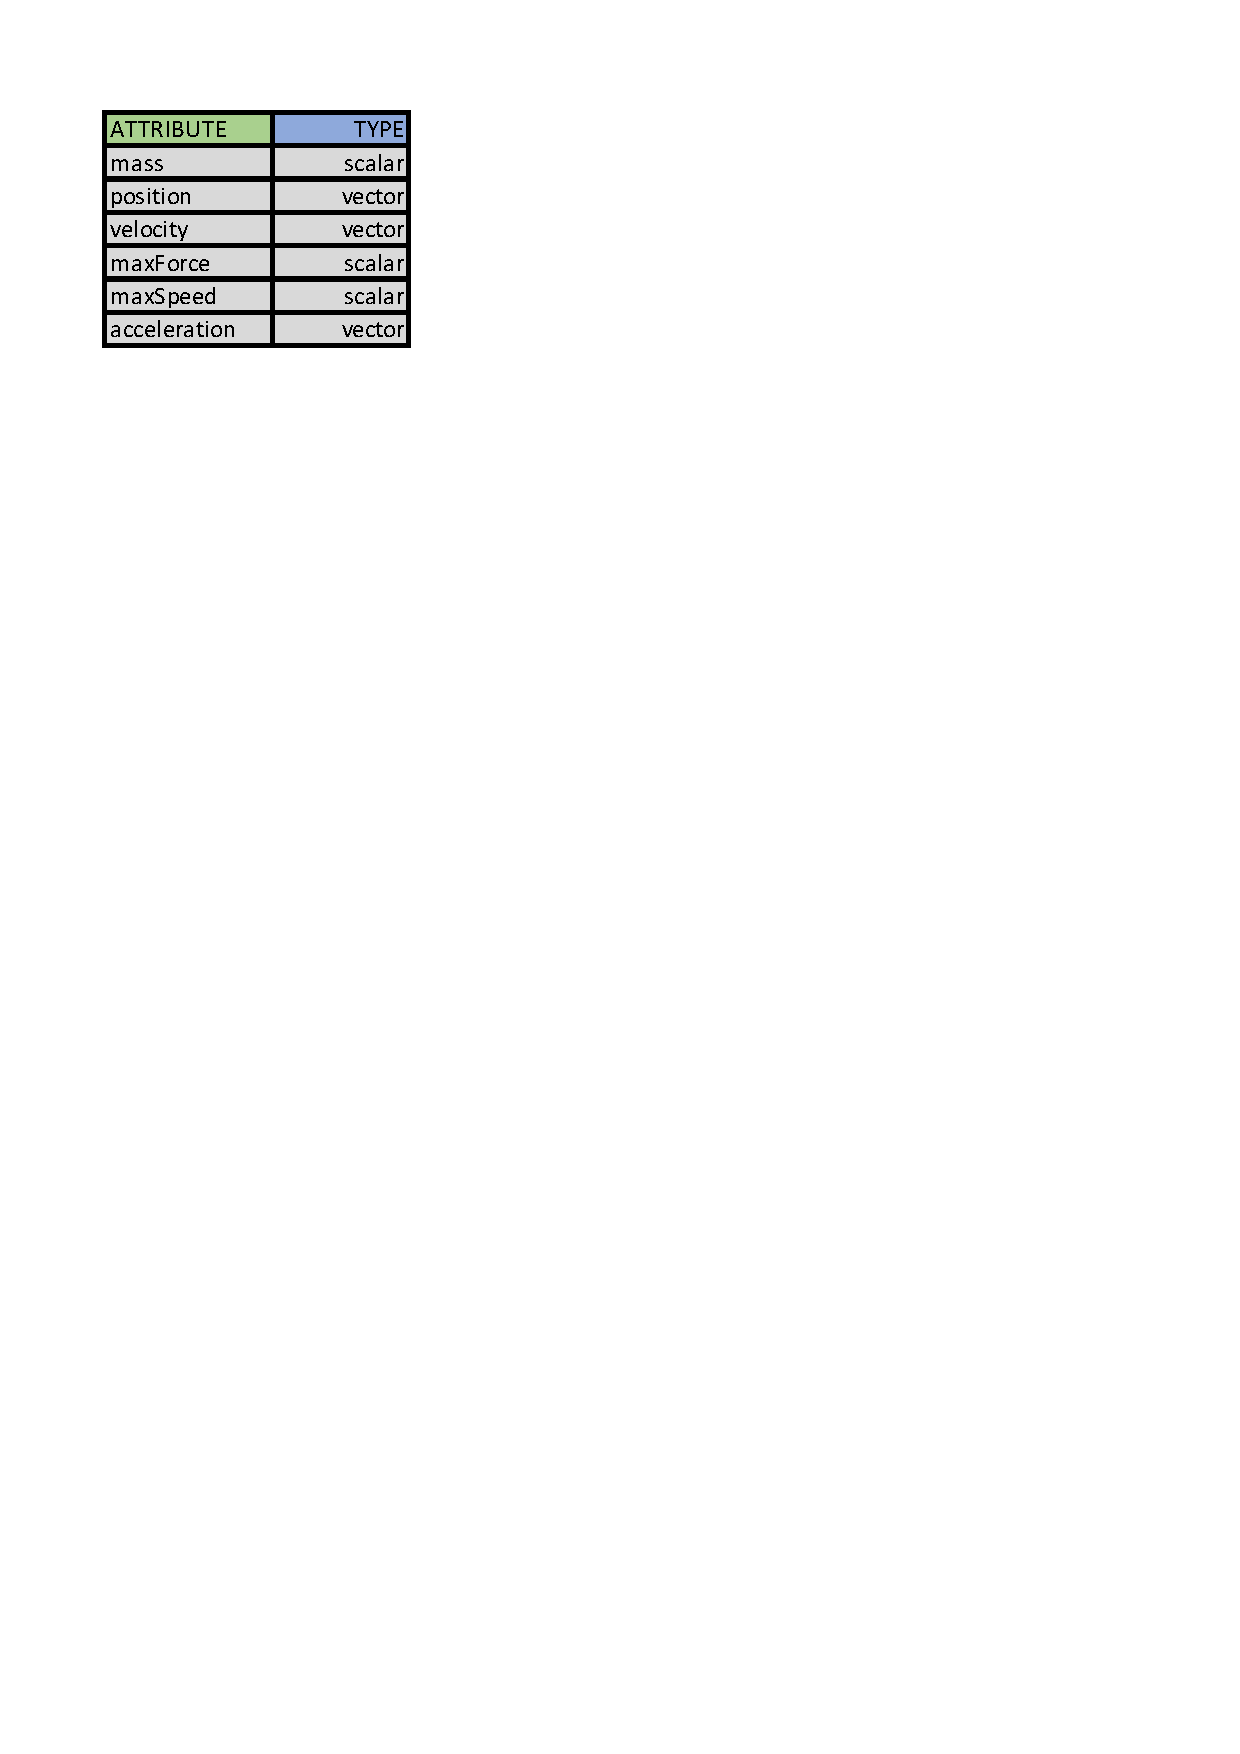
\includegraphics[scale=0.6]{attributes.pdf}

\textbf{Important note} - Most characters have a maximum speed they can travel; 
they can’t accelerate indefinitely. The maximum can be
explicit, held in a variable or constant. (\cite{Millington} chapter 3.3.3.)

\subsection{Characteristics of seek and arrive } \label{characterictics of seek and arrive}

\subsubsection{Seek} \label{seek}

Seeking steers a character towards a specified position in space. 
This behavior aligns the vector of a velocity toward the target. 
But how do we calculate the steering force if we do not want the 
vehicle to steer completely right after seeing the target? We can 
diagram our problem from \ref{problem to solve}.

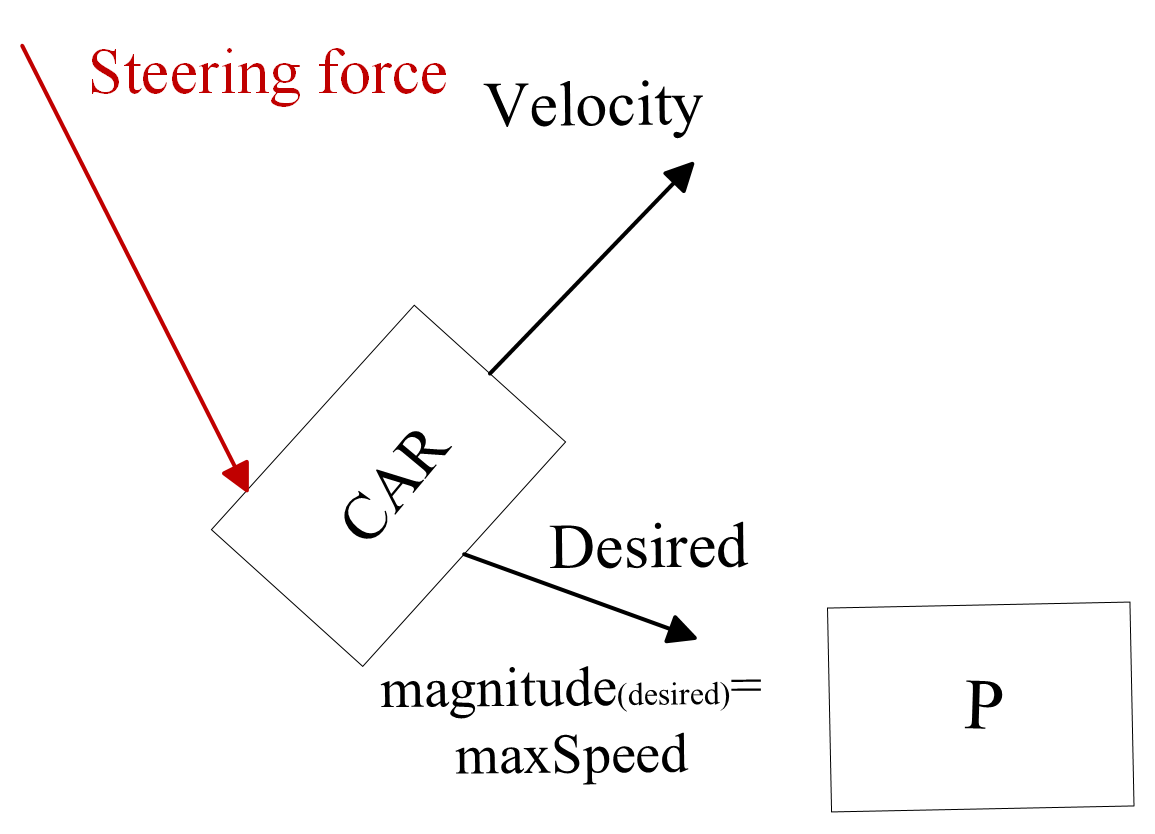
\includegraphics[scale=0.22]{diagram_car.png} 	
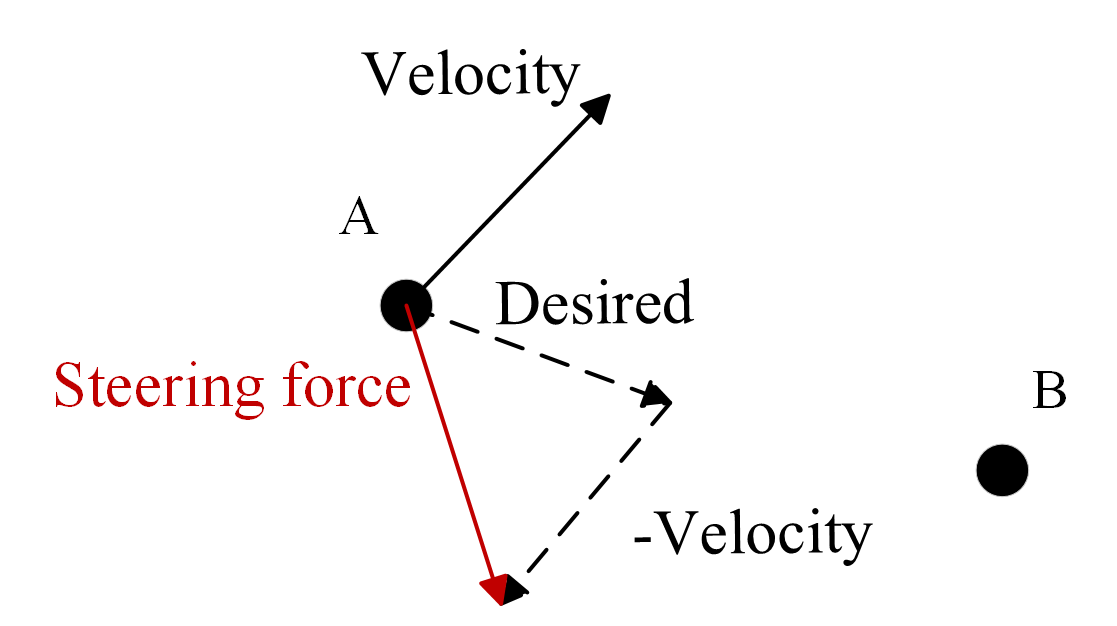
\includegraphics[scale=0.22]{diagram_steeringForce.png}\par
\quad Figure 2 
\hspace*{\fill} Figure 3
\bigbreak

The steering force is then calculated with this formula * as shown 
in the Figure 3.

\begin{center}
$desired =position A - position B \quad (vectors)$ \par
$ *steering force= desired – velocity$

\end{center}

As we are designing the animation, the steering force is updated with 
each frame and has a lower effect next time each time it is applied. 
The vector of velocity is aligned with the desired one
more and more with every frame.

\subsubsection{Arrive} \label{arrive}

When we want to simulate arrival, we must think about gradually 
decreasing the speed of the vehicle and eventually stopping it once the 
vehicle passes some imaginary boundary. The following diagram describes 
the situation. 

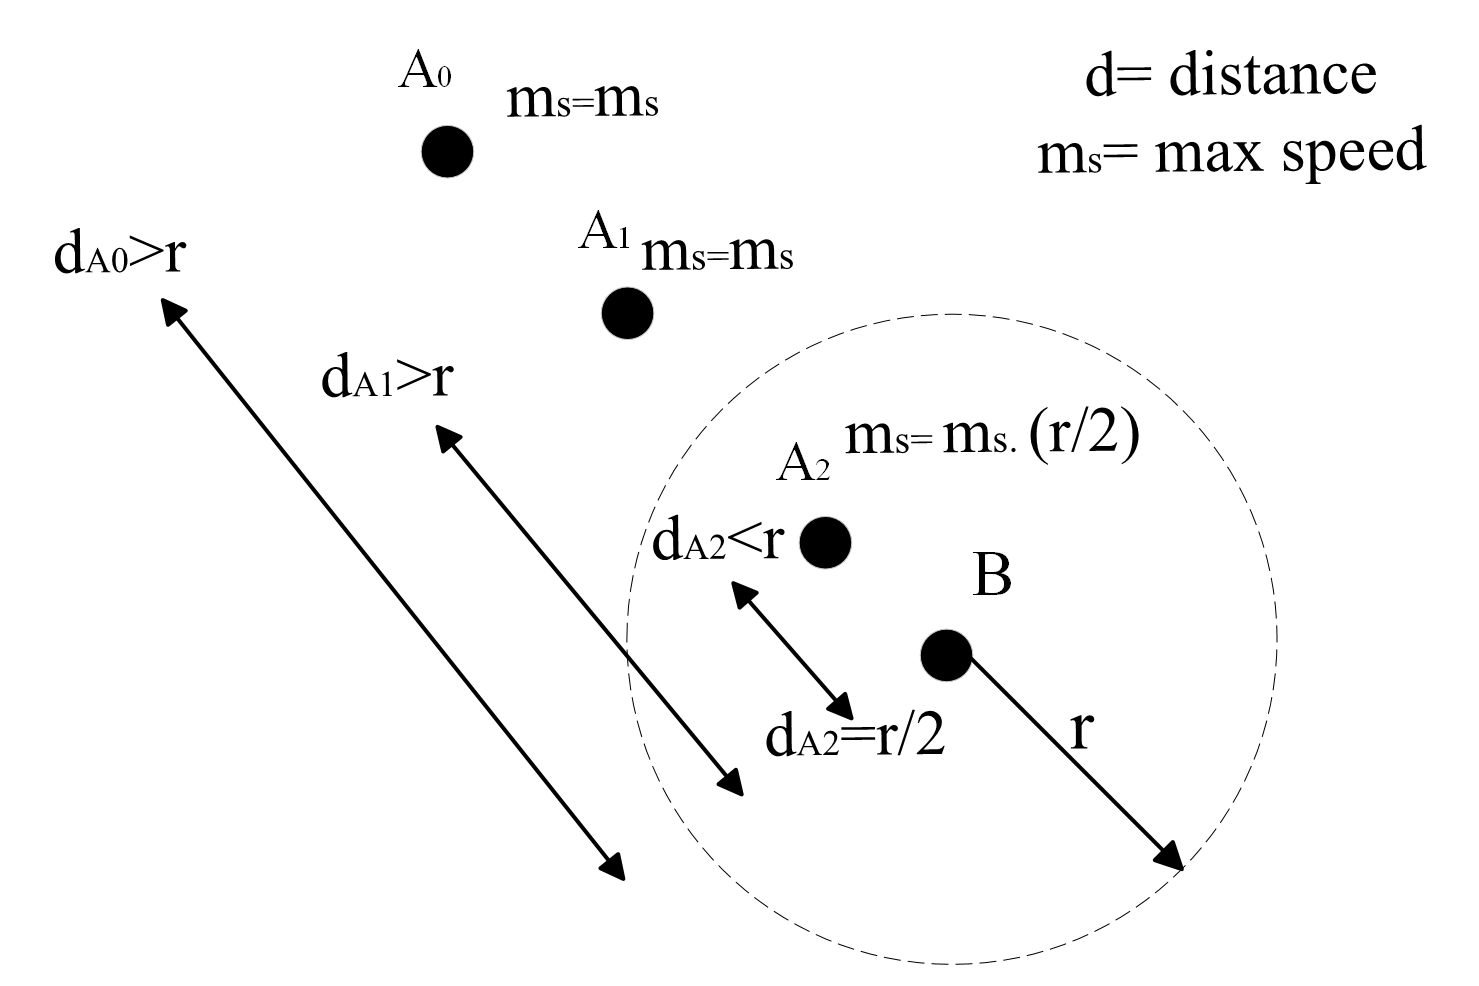
\includegraphics[scale=0.22]{diagram_radius.png}\par
Figure 4
\bigbreak
From the Figure 4 we can assume two things: 

\begin{center}
$d>r 	\Rightarrow speed = maxSpeed$ \par 
$d \leq r \Rightarrow speed = (d/r)  . maxSpeed$ 
\end{center} 

From the second equation we can see that once the object passes through
the circle of the radius r, the speed is decreasing in a fraction of 
the distance $d$ and radius $r$. Once we have the new \textbf{lower} 
speed calculated, then the magnitude of a vector of the desired velocity is set
to the size of that lower max speed. The closer to the place of stopping,
the lower the speed is.

\section{Simulating the behavior in p5.js} \label{simulation} 

The objective of this project was to simulate the behavior. This chapter briefly
introduces the tool that was used and explains the main parts of the code. There is also a short 
commentary to a time complexity of the algorithm included.\\
For the link to the animation \textbf{\underline{\href{https://editor.p5js.org/RichardCernansky/sketches/E0zAXshWw}{click here}}}.

\subsection{What is p5.js?} \label{p5 char} 

p5.js is a JavaScript library for creative coding, with a focus on 
making coding accessible and inclusive for artists, designers, or 
educators. It is a collection of pre-written code and provides us 
with tools that simplify the process of creating interactive visuals 
with code in the web browser. p5.js is free and open source. We 
will use it for creating the animation from \ref{problem to solve}. 

\subsection{Main part of the code - class Vehicle and its functions} \label{class Vehicle} 

\subsubsection{constructor() function} \label{constructorf} 

This function creates all the variables for values that were stated in the 
chapter \ref{types of behaviors} (the variable for mass is missing because we do not change it in animation
so it will not affect it). As an input, it gets updated $x$ and $y$ position
of the vehicle. 

\subsubsection{seek() function} \label{seekf} 

Seek function gets as an input vector Target representing $x$ and $y$ position
of the target. First, it calculates the steering force by subtracting velocity vector
from desired velocity vector (\ref{seek}). An $if$ statement included in a function checks if 
the distance is lower than 100 pixels. If yes, then it sets the magnitude of the 
desired velocity to some portion of max speed accordingly to the distance. 
Otherwise, it sets the magnitude to the size of max speed.

\subsubsection{update() function} \label{updatef} 

The update function applies the steering force combined with velocity to the vehicle
in every frame. The result is our realistically-looking steering animation. 

\subsection{Time complexity} \label{time complexity} 

The time complexity of a seeking steering behavior algorithm 
for one object and one target is O(1), meaning that the 
calculation time remains constant regardless of the number 
of objects being simulated. This is because seeking is a 
low-complexity steering behavior algorithm that only 
requires a few simple calculations to determine the steering 
force for a single object. The calculations involved in 
seeking are relatively simple and do not depend on the 
number of objects being simulated, so the calculation time 
remains constant.

\section{Research method and literature review} \label{research method} 

The source article \cite{Raynolds} is what introduced me to the topic. 
From the beginning of my research, there were a lot of questions. 
The idea of an autonomus agent was mentioned in Raynold's article
but to completely understand it, I had to search deeper. A part of the book Vehicles 
\cite{Braitenberg} and the article from Verhangen \cite{Verhagen} gave me a complete
understanding. 

Raynold's article is what also helped me the most with coming up with formulas for
the calculation of the steering force. The explanation of his ideas is clear and 
understandable for anyone with a knowledge of coordinate geometry 
and the physics of forces. 

\section{Result} \label{results} 

After stating a problem in \ref{problem to solve}, the result of this 
project was made clear. We wrote a code for a realistic animation of seek and arrive
steering behavior using knowledge of forces, and vectors and operating with them.  
This can be used in in-game graphics for creating self-controlled worlds 
of objects that move according to an algorithm they obey. The player 
has then a better artistic experience from their motion because it looks 
natural and unpredictable. 

\section{The technology and people} \label{technology and people} 

Technology and people often intersect in the realm of steering behaviors.
Steering behaviors are a core part of many types of technology, from animations in games,
to self-driving cars, drones or virtual assistants and robots. 
These technologies rely on algorithms and sensors to gather information about 
their surroundings and make decisions based 
on that information, enabling them to move and interact with the world 
in intelligent and adaptive ways. 

At the same time, if we consider the basic idea of autonomous agents,
we could think of it as an important aspect of human psychology and sociology, as 
people constantly make decisions and adjust their behavior in response to their 
environment. This could help us 

\section{Sustainability question} \label{sustainability} 

Sustainability in animations in games is becoming an increasingly important 
issue in the industry. As animation technology becomes more advanced, the amount 
of computing power and energy required to create and run animations in games has 
increased. This has led to concerns about the environmental impact of animations 
in games and the need for more sustainable practices. 
Game developers are working to reduce the environmental impact of their animations
by using more efficient 
algorithms and hardware, as well as by implementing strategies for reducing the 
energy consumption of their games. 

Additionally, some game developers are 
incorporating sustainability themes into their games to raise awareness about 
the importance of sustainability among players. 
According to a research by
Rajamangala University of Technology in Thailand \cite{phong}, the very efficient way for 
people to learn manners of sustainability is by playing video games during 
the age of primary education when the information delivered through the games 
remains among most of the children for the rest of their lives.

\section{Conclusion} \label{conclusion}

To sum up, the goal of this project was to animate seek and arrival 
steering behavior in two dimensions. The challenge was to 
make it look as realistic as possible. Firstly, we came 
up with the formulas to calculate the steering force using 
physics. We did not want the vehicle to be able to 
steer immediately and rush at full speed to the target. Instead, 
we wanted to make the animation smooth, which was done. 

The second challenge was to make the vehicle eventually stop after 
reaching the target. The idea of gradually slowing down after 
crossing a boundary works perfectly. The last part was to put the ideas
for steering into an algorithm that animated such behavior. 

Although I succeeded in creating a certain type of steering behavior,
there are still many to be invented. For example, complicated group behaviors
follow up on this topic. Also considering the three-dimensional space
and inventing reality-based models is still an open topic to be explored
and can be used both in games and reality for the motion of 
self-driving cars.



\section*{Acknowledgement}
I would like to thank my friend Lukáš Častven for introducing 
the problem to me and arousing my interest in the topic\ldots

\bibliography{literatura} 
\bibliographystyle{plain}  

\end{document} 

